\section{Temporal Smoothness}

Besides the odd-one-out question, temporal smoothness can be exploited to learn high-level concepts from unlabeled video.
This is motivated by dimensionality reduction, which aims to translate high dimensional data to a low dimensional representation such that similar input objects are mapped to nearby points in feature space. 
In this this section, we first provide a breif review of a temporal smoothness prior that is first used in a dimension reduction algorithm called Dimensionality Reduction by Learning an Invariant Mapping (DrLIM)\cite{LeCun2006DrLIM}. Then we present several improvements on the prior and fit it in our problem. 

Consider a set of input vectors $I = \{x_1, ..., x_p\}$ and a parametric function $G_W$ returns extracted features. 
For each $x_i \in I$ there exist a subset of vectors in $I$ that are deemed as similar to $x_i$.  
Let $x_1, x_2 \in I$ be a pair of input vectors and $Y$ be a binary label assigned to this pair.
$Y = 0$ if $x_1$ and $x_2$ are deemd similar, and $Y = 1$ if they are deemed dissimilar.
Define the parameterized distance function to be learned $D_W$ between $x_1, x_2$ as the euclidean distance between the outputs of $G_W$ . 
That is,
$$D_W(x_1, x_2) = || G_W(x_1) - G_W(x_2)||_2$$
To shorten notation, $D_W (x_1, x_2)$ is written as $D_W$ . Then the proposed loss function is
$$L(W) = \sum_i L(W, (Y, x_1, x_2)^i) $$
$$L(W, (Y, x_1, x_2)^i) = (1-Y) L_S (D_W^i) + Y L_D (D_W^i)$$
where $(Y, x_1, x_2)^i$ is the $i$-th labeled sample pair, $L_S$ is the partial loss function for a pair of similar points, $L_D$ the partial loss function for a pair of dissimilar points. 

$L_S$ and $L_D$ must be designed such that minimizing $L$ with respect to $W$ would result in low values of $D_W$ for similar pairs and high values of $D_W$ for dissimilar pairs. In specific, they can be designed as following 
$$L_S (D_W^i) = \frac{1}{2} (D_W)^2$$
$$L_D (D_W^i) = \frac{1}{2} (max\{0, m - D_W\})^2$$
Figure~\ref{fig:twoloss} shows these two loss functions. Then the total loss function is 
$$L(W, Y, x_1, x_2) = (1-Y) \frac{1}{2} (D_W)^2 + (Y) \frac{1}{2} (max\{0, m - D_W\})^2$$

\begin{figure}
\centering
\hspace{-3mm}
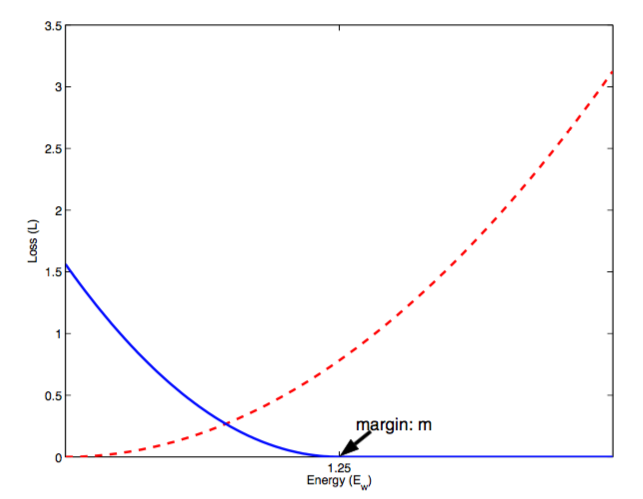
\includegraphics[width=0.4\textwidth]{./Images/twoloss.png}
\caption{Graph of the loss function $L$ against the energy $D_W$. The dashed (red) line is the loss function for the similar pairs and the solid (blue) line is for the dissimilar pairs.}
\label{fig:twoloss}
\vspace{-4mm}
\end{figure}

This loss formalization can be directly implemented in temporal coherence. Consider $x_t$ and $x_t\rq{}$ are input frames at two different times, then smoothness loss for a single sample pair can be written as:\\
$L_T(x_t, x_t\rq{}, W) = $
\[   
     \begin{cases}
       ||G_W(x_t) - G_W(x_t\rq{})||_p & \text{if} |t-t\rq{}| = 1\\
       max(0, m - ||G_W(x_t) - G_W(x_t\rq{})||_p) &\text{if} |t-t\rq{}| > 1 \\
     \end{cases}
\]

The margin $m$ is introduced to avoid the degenerate solution $G_W(x_t) = G_W(x_0)$ for all $t$. 
Specifically, this margin term encourages data samples that are not temporal neighbors to be separated by at least a distance of $m$-units in feature space. 

However, the second contrastive term in loss $L_T(x_t, x_t\rq{}, W)$ only depends on pairwise distances in the feature space, and hence does not guarantee that the resulting feature space is informative with respect to the input. 
One improvement is to replace this contrastive term with a term that penalizes the reconstruction error of both data samples \cite{LeCun2014coherence}. 
This reconstruction term not only prevents the constant solution but also acts to explicitly preserve information about the input.

Another improvement is to extract temporal slow features by applying pooling operators in feature space. 
In natural video and on small spatial scales these features mainly correspond to local translations and deformations. 
Invariances to such changes can be achieved using appropriate pooling operators \cite{Mallat2013scattering}.
We divide each feature vector into $K$ potentially overlapping neighborhoods and denote each of them as $P_i$. 
Specifically, we apply L2-Pooling and the loss discussed above can be expressed as following:
$$L_T(x_t, x_t\rq{}, W) = \sum_{\tau = \{t, t\rq{}\}} (||W_d G_W(x_\tau) - x_\tau||^2 + \alpha |G_W(x_\tau)|)$$
$$+ \beta \sum_{i=1}^K |||G_W(t)||^{P_i} -  ||G_W(t\rq{})||^{P_i}|$$